% +--------------------------------------------------------------------+
% | LaTeX Template                                                     |
% | for K-State Electronic Theses, Dissertations, and Reports          |
% |                                                                    |
% | Comments and guidelines for using the template are shown           |
% | within boxes like this one.                                        |
% |                                                                    |
% | Revised 6/30/06                                                    |
% | 9/14/06: Removed typos                                             |
% +--------------------------------------------------------------------+

% +--------------------------------------------------------------------+
% | Your paper should contain the following sections, except where     |
% | indicated as optional, in the order shown.  Also, all headings     |
% | shown with an asterisk (*) must be centered and in uppercase       |
% | letters:                                                           |
% |                                                                    |
% | Abstract Title Page (doctoral dissertations only)                  |
% | ABSTRACT* (doctoral dissertations only)                            |
% | Title Page                                                         |
% | Copyright Page (Optional - only needed if copyrighting)            |
% | ABSTRACT *                                                         |
% | TABLE OF CONTENTS *                                                |
% | LIST OF FIGURES *                                                  |
% | LIST OF TABLES*                                                    |
% | ACKNOWLEDGMENTS* (Optional)                                        |
% | DEDICATION * (Optional)                                            |
% | PREFACE * (Optional)                                               |
% | Individual Chapters                                                |
% | References and/or bibliography                                     |
% | Appendices (as needed)                                             |
% +--------------------------------------------------------------------+

% +--------------------------------------------------------------------+
% | The LaTex keyword \documentclass selects a particular class to     |
% | associate with the document.  The current documentclass            |
% | {class_diss} generates a Table of Contents that has leading dots   |
% | only on chapter subheadings.  If you prefer a Table of Contents    |
% | that has leading dots for all entries, replace {class_diss}        |
% | with {Mydiss} in the command below.                                |
% |                                                                    |
% +--------------------------------------------------------------------+

\documentclass[final, 12pt,oneside]{class_diss}

% +--------------------------------------------------------------------+
% | The following command sets the bibliography style to American
% | Institute of Physics (AIP).  Other styles are available in the
% | styles directory.  To use a different style, replace "aip" with
% | the filename of the style you want to use.
% +--------------------------------------------------------------------+

%\bibliographystyle{styles/plain}

\usepackage[utf8]{inputenc}
\usepackage[T1]{fontenc}
\usepackage[spanish]{babel}
\selectlanguage{spanish}
\usepackage{eurosym}


% +--------------------------------------------------------------------+
% | Now, we add in all external packages that we will use throughout   |
% | the document.  You can add other packages as needed.
% +--------------------------------------------------------------------+

%\usepackage{     caption2} % Customize captions a bit more
\usepackage{      amsmath} % American Mathematics Society standards
%\usepackage{      wrapfig} % Wraps text around a figure or table
\usepackage{     graphicx} % Extended graphics package.
%\usepackage{     fancyhdr} % Efficiently handles headers and footers
%\usepackage{       braket} % Bra-Ket notation package
%\usepackage{     mathrsfs} % Specialized Math fonts (Hamiltonian, etc.)
%\usepackage{boxedminipage} % Boxed text can be produced
%\usepackage{     setspace} % Controls line spacing via \begin{space}
%\usepackage{svg}
%\usepackage[dvips]{graphicx} 
\usepackage{subfigure}
\usepackage{amsxtra}
\usepackage{amssymb}
\usepackage{amsthm}
\usepackage{latexsym}
\usepackage{amsmath}


\usepackage{enumerate}
\usepackage{float}

% +--------------------------------------------------------------------+
% | The color package allows one to select colors for hyperlinking     |
% | (see below).                                                       |
% +--------------------------------------------------------------------+

\usepackage[usenames]{color}
\usepackage{pgfgantt}

% +--------------------------------------------------------------------+
% | Colors defined for use with this template.                         |
% +--------------------------------------------------------------------+

\definecolor{  Pink}{rgb}{1.0, 0.5, 0.5}
\definecolor{Maroon}{rgb}{0.8, 0.0, 0.0}

% +--------------------------------------------------------------------+
% | In the commands below, we use the 'natbib' package, and specify    |
% | the 'sort&compress' option, which condenses                        |
% | citations from (1,2,3,5,9,10,11) to (1-3,5,9-11).  The 'bibpunct'  |
% | option selects various parameters for how the citation will be     |
% | displayed.  In this case, only the comma (separation between       |
% | citations) and the 's' (superscript) arguments are chosen.  The    |
% | other curly braces deal with how to 'wrap' the citation (using     |
% | parentheses, brackets, etc.) and are not needed for the chosen     |
% | style.                                                             |
% +--------------------------------------------------------------------+
%\usepackage[numbers]{natbib}
\usepackage[numbers,sort&compress]{natbib}
%\bibpunct{}{}{,}{s}{}{}
%\usepackage{hypernat}

% +--------------------------------------------------------------------+
% | Lastly, the hyperref package allows one to hyperlink cross-        |
% | references and figures in a LaTeX document.                        |
% +--------------------------------------------------------------------+

\usepackage[pdftex, plainpages=false, pdfpagelabels]{hyperref}
\usepackage{url}
\usepackage{listings}
%\usepackage{minted}
\hypersetup{
    linktocpage=true,
    colorlinks=true,
    bookmarks=true,
    citecolor=blue,
    urlcolor=red,
    linkcolor=Maroon,
    citebordercolor={1 0 0},
    urlbordercolor={1 0 0},
    linkbordercolor={.7 .8 .8},
    breaklinks=true,
    pdfpagelabels=true,
    }

% +--------------------------------------------------------------------+
% | Page margins are set on 1 inch on all sides.                       |
% +--------------------------------------------------------------------+

\topmargin      = -0.56in
\textheight     =  8.60in
\textwidth      =  6.46in
\oddsidemargin  =  0.02in

% +--------------------------------------------------------------------+
% | The document finally begins here.                                  |
% +--------------------------------------------------------------------+

\begin{document}


  \setcounter{page}{-1}


% +--------------------------------------------------------------------+
% | Title Page -- Required for both Doctoral and Masters Students
% +--------------------------------------------------------------------+

% +--------------------------------------------------------------------+
% | Title Page
% +--------------------------------------------------------------------+

\newpage

% +--------------------------------------------------------------------+
% | This page should not contain a page number.  We use the
% | \thispagestyle[empty] command below to suppress page numbers
% | and other style elements.
% +--------------------------------------------------------------------+

\thispagestyle{empty}

% +--------------------------------------------------------------------+
% | The Title page begins here.
% +--------------------------------------------------------------------+

\begin{center}

   \vspace{1cm}

% +--------------------------------------------------------------------+
% | On the line below, replace "ENTER YOUR TITLE" with the title of
% | your ETDR.  Use all CAPITAL LETTERS.
% +--------------------------------------------------------------------+

   {\Large \textbf{UNIVERSIDAD COMPLUTENSE DE MADRID}}\\

   \vspace{0.3cm}
   {\Large FACULTAD DE CIENCIAS FÍSICAS}\\
   \vspace{0.3cm}
   {DEPARTAMENTO DE ARQUITECTURA DE COMPUTADORES Y AUTOMÁTICA}\\

   

   \vspace{0.65cm}
   \rule{2in}{0.5pt}\\
   \vspace{0.85cm}

\vspace{0.5cm}

  
\includegraphics[height=2.4in]{figures/escudo.jpg}

   \vspace{0.5cm}  
  {\large \textbf{TRABAJO DE FIN DE GRADO}}\\ 

  \vspace{0.3cm} 

  \textbf{Código TFG: [Código TFG]}\\
  
   \vspace{0.5cm}
     
%+-- Escribe el nombre de tu Trabajo de Fin de Grado
  \textbf{[Desarrollo de sistemas de control cooperativos para USVs en tareas de bioinspección]}\\
  \vspace{0.3cm}  
  \textbf{[Cooperative Control Systems for USVs in Bio-surveillance tasks]}
% +--------------------------------------------------------------------+

   \vspace{1.2cm}

% Nombre del alumno y datos de la convocatoria:   
  [Ulises Alejandro Ardizzi Rodríguez]\\

   \vspace{1.2cm}
% Supervisores o directores del trabajo:
  Supervisor/es: [Nombre del/os supervisores]
% +--------------------------------------------------------------------+   
  
  \vspace{2.5cm}
  Grado en Ingeniería Electrónica de Comunicaciones\\
  Curso académico 20[XX-XX]\\
  Convocatoria XXXX\\



\end{center}

%{\raggedleft
%Directores:\\
%   \vspace{ 1cm}
%Apellidos, Nombre\\
%Apellidos, Nombre\\
%}


% +--------------------------------------------------------------------+
% | Use the section below if you have co-major professors.
% +--------------------------------------------------------------------+

%\begin{flushleft}
%   \hspace{10cm}Approved by:\\
%   \vspace{ 1cm}
%   \hspace{10cm}Co-Major Professor\\
%   \hspace{10cm}Enter Your Co-Major Professor's Name\\
%   \vspace{.5cm}
%   \hspace{10cm}Co-Major Professor\\
%   \hspace{10cm}Enter Your Co-Major Professor's Name\\
%\end{flushleft}

   \pdfbookmark[0]{Portada}{PDFPortadaPage}

% +--------------------------------------------------------------------+
% | Autorizacion Page -- Required for both Doctoral and Masters Students
% +--------------------------------------------------------------------+
% +--------------------------------------------------------------------+
% | Copyright Page
% +--------------------------------------------------------------------+
% 
\newpage
\thispagestyle{empty}
\mbox{}
\newpage

\thispagestyle{empty}

\begin{center}

{\bf \Huge Autorización de difusión}

\vspace{1cm}

% +--------------------------------------------------------------------+
% | On the line below, replace "Enter Your Name" with your name Use the same
% | form of your name as it appears on your title page. Use mixed case, for
% | example, Lori Goetsch.
% +--------------------------------------------------------------------+
% 
   \large Apellidos, Nombre\\

   \vspace{0.5cm}

% +--------------------------------------------------------------------+
% | On the line below, replace Fecha
% | % |
% +--------------------------------------------------------------------+
% 
   Madrid, a XX de XX de XX\\

   \vspace{0.5cm} \end{center}

Los abajo firmantes, matriculados en el Grado de XX de la
Facultad de XX, autorizan a la Universidad Complutense de Madrid (UCM) a
difundir y utilizar con fines académicos, no comerciales y mencionando
expresamente a su autor el presente Trabajo Fin de Grado: “Título”, realizado
durante el curso académico XX-XX bajo la dirección de XX y la co-dirección de XX en el Departamento de XX, y a la
Biblioteca de la UCM a depositarlo en el Archivo Institucional E-Prints
Complutense con el objeto de incrementar la difusión, uso e impacto del trabajo
en Internet y garantizar su preservación y acceso a largo plazo.

{
\begin{center}
\vfill

\includegraphics{figures/cc-by-nc-sa.png}
\tiny

Esta obra está bajo una\\
\href{http://creativecommons.org/licenses/by-nc-sa/4.0/}{Licencia Creative Commons\\Atribución-NoComercial-CompartirIgual 4.0 Internacional}.
\end{center}
}
   \pdfbookmark[0]{Autorización}{PDFAutorizacionPage}


% +--------------------------------------------------------------------+
% | Dedication Page
% |
% | If you choose not to have a Dedication page, comment out
% | or delete the following 3 lines.
% +--------------------------------------------------------------------+

%\newpage
\vspace{1cm}
\setlength{\baselineskip}{0.8cm}

\begin{flushright}
\textit{``Dedicatoria, si es necesaria.''
}\\
Edward Tufte
\end{flushright}
%\phantomsection
%\addcontentsline{toc}{chapter}{Dedicatoria}

   % +--------------------------------------------------------------------+
% | Acknowledgements Page
% |
% | If you choose not to have an Acknowledgements page, comment out
% | or delete the following 3 lines.
% +--------------------------------------------------------------------+
\pagenumbering{roman}
\setcounter{page}{1}
\newpage
\setlength{\parindent}{0cm}
\begin{center}
{\bf \Huge Agradecimientos}
\end{center}
\vspace{1cm}
\setlength{\baselineskip}{0.8cm}

En primer lugar, a Héctor García de Marina y Juan Francisco Jiménez Castellanos por su dedicación a lo largo de estos meses para llevar a cabo este proyecto. Siempre que tenía una duda o necesitaba algo en particular estaban en disponibilidad para ayudarme, además han contribuido en mi crecimiento tanto personal como profesional.

\vspace{0.5cm}

Agradecer sobretodo a mi familia, más concretamente mis dos padres por el apoyo, tiempo dedicado y esfuerzo para que pueda estudiar con todas las facilidades del mundo. Se que no soy muy expresivo pero estoy muy agradecido por todo lo que han hecho por mi.

\vspace{0.5cm}

Por último, agradecer a mis amigos más cercanos que han estado siempre ahí para apoyarme y ayudarme en todo momento que lo necesitaba.

\vspace{0.5cm}

Se que no he puesto muchas cosas, pero soy una persona que considera los agradecimientos en papel dado que se sienten como palabras vacias, creo que es mejor demostrar el agradecimiento con acciones.
\phantomsection
%\addcontentsline{toc}{chapter}{Agradecimientos}

% +--------------------------------------------------------------------+
% | We use the following code to suppress page numbers and other
% | style issues we do not want present on a given page.               |
% +--------------------------------------------------------------------+

%\thispagestyle{empty} Looks like it's ok to remove this line
\newpage

% +--------------------------------------------------------------------+
% | On the line below, set the number to represent the page number of
% | the Table of Contents page.  For example, if the Table of Contents
% | page is the 8th page of your document, enter 8 in the brackets.  This
% | number may vary, depending on the length of your abstract.
% |
% | Numbers do not appear on the title and abstract pages, but they are
% | included in the page count.  The Table of Contents page is the
% | first page on which page numbers are displayed.
% +--------------------------------------------------------------------+


% +--------------------------------------------------------------------+
% | Preface Page (Prologo)
% +--------------------------------------------------------------------+

%% EN PRINCIPIO NO LO USAMOS

% +--------------------------------------------------------------------+
% | Preface (Optional)
% +--------------------------------------------------------------------+

\newpage
\begin{center}
{\bf \Huge Preface}
\end{center}
\vspace{1cm}
\setlength{\baselineskip}{0.8cm}

%\pdfbookmark[0]{Preface}{PDF_Preface}

% +--------------------------------------------------------------------+
% | Enter text of your Preface in the space below this box.
% +--------------------------------------------------------------------+

This template uses a separate file for each section of your ETDR:
title page, abstract, preface, chapters, reference, etc.  This
makes it easier to organize and work with a lengthy document.  The
template is configured with page margins required by the Graduate
School and will automatically create a table of contents, lists of
tables and figures, and PDF bookmarks.

Although the template gives you a foundation for creating your
ETDR, you will need a working knowledge of LaTeX in order to
produce a final document.  You should be familiar with LaTeX
commands for formatting text, equations, tables, and other
elements you will need to include in your ETDR.

This template uses a separate file for each section of your ETDR:
title page, abstract, preface, chapters, reference, etc.  This
makes it easier to organize and work with a lengthy document.  The
template is configured with page margins required by the Graduate
School and will automatically create a table of contents, lists of
tables and figures, and PDF bookmarks.

Although the template gives you a foundation for creating your
ETDR, you will need a working knowledge of LaTeX in order to
produce a final document.  You should be familiar with LaTeX
commands for formatting text, equations, tables, and other
elements you will need to include in your ETDR.

This template uses a separate file for each section of your ETDR:
title page, abstract, preface, chapters, reference, etc.  This
makes it easier to organize and work with a lengthy document.  The
template is configured with page margins required by the Graduate
School and will automatically create a table of contents, lists of
tables and figures, and PDF bookmarks.

Although the template gives you a foundation for creating your
ETDR, you will need a working knowledge of LaTeX in order to
produce a final document.  You should be familiar with LaTeX
commands for formatting text, equations, tables, and other
elements you will need to include in your ETDR.

%\phantomsection
%\addcontentsline{toc}{chapter}{Preface}

% +--------------------------------------------------------------------+
% | Here, we will generate our Table of Contents (TOC) entries.        |
% | This adds the section to the TOC and then generates the indicated  |
% | section.                                                           |
% +--------------------------------------------------------------------+

%\addcontentsline{toc}{chapter}{Resumen}
\pdfbookmark[0]{Resumen}{PDFResumenPage}
% +--------------------------------------------------------------------+
% | Copyright Page
% +--------------------------------------------------------------------+

\newpage

\thispagestyle{empty}

{\bf \large [Título extendido del TFG (si procede)]}

\vspace{0.5cm}

{\bf \large Resumen}\\
Breve resumen de contenidos.


\vspace{5cm}


{\bf Palabras clave:}


   
   Separadas, por, comas.
   
   \vspace{1 cm}


{\bf \large Abstract}\\

\vspace{5cm}

{\bf Key works:}

% ------------- Para eliminar ----------
\vspace{0.9cm}
\begin{center}
[Nota: el título extendido (si procede), el resumen y abstract deben estar en una misma página y su extensión no debe superar la página. Tamaño mínimo 11 pto.\\

Extensión máxima 50 páginas sin contar portada ni resumen (sí se incluye índice, introducción, conclusiones y bibliografía)]\\
\end{center}
% ----------------------------------------
  
\newpage

\phantomsection
%\addcontentsline{toc}{chapter}{Índice}

\tableofcontents
\listoffigures
%\listoftables

%\hfill  Are these lines necessary?
%\hfill

%\newpage
%\addcontentsline{toc}{chapter}{Resumen}
%\pdfbookmark[0]{Resumen}{PDFResumenPage}
%% +--------------------------------------------------------------------+
% | Copyright Page
% +--------------------------------------------------------------------+

\newpage

\thispagestyle{empty}

{\bf \large [Título extendido del TFG (si procede)]}

\vspace{0.5cm}

{\bf \large Resumen}\\
Breve resumen de contenidos.


\vspace{5cm}


{\bf Palabras clave:}


   
   Separadas, por, comas.
   
   \vspace{1 cm}


{\bf \large Abstract}\\

\vspace{5cm}

{\bf Key works:}

% ------------- Para eliminar ----------
\vspace{0.9cm}
\begin{center}
[Nota: el título extendido (si procede), el resumen y abstract deben estar en una misma página y su extensión no debe superar la página. Tamaño mínimo 11 pto.\\

Extensión máxima 50 páginas sin contar portada ni resumen (sí se incluye índice, introducción, conclusiones y bibliografía)]\\
\end{center}
% ----------------------------------------
  

%   % +--------------------------------------------------------------------+
% | Copyright Page
% +--------------------------------------------------------------------+

\newpage

\thispagestyle{empty}

\begin{center}

{\bf \Huge Resumen}

  \end{center}
\vspace{1cm}

La robotica de enjambre 

\vspace{1cm}

% +--------------------------------------------------------------------+
% | On the line below, repla	ce Fecha
% |
% +--------------------------------------------------------------------+

\begin{center}

{\bf \Large Palabras clave}

   \end{center}

   \vspace{0.5cm}
   
   Separadas, por, comas.
   




%   \addcontentsline{toc}{chapter}{Resumen}
%   \pdfbookmark[0]{Resumen}{PDFResumenPage}

%    % +--------------------------------------------------------------------+
% | Copyright Page
% +--------------------------------------------------------------------+

\newpage

\thispagestyle{empty}

\begin{center}

{\bf \Huge Abstract}

  \end{center}
\vspace{1cm}


 
\vspace{1cm}

% +--------------------------------------------------------------------+
% | On the line below, replace Fecha
% |
% +--------------------------------------------------------------------+

\begin{center}

{\bf \Large Keywords}

   \end{center}

   \vspace{0.5cm}
   
Separadas, por, comas.
   



%       \addcontentsline{toc}{chapter}{Abstract}
%       \pdfbookmark[0]{Abstract}{PDFAbstractPage}
%   \vfill
    
    



% +--------------------------------------------------------------------+
% | We use arabic (1, 2, 3...) page numbering starting from page 1.    |
% | Note, however, that there are many pages where this is not the     |
% | desired behavior - such as the Title page, or abstract.  In these  |
% | cases, we can use \thispagestyle{empty} to suppress page numbers,  |
% | and other general style issues that we've defined globally.        |
% +--------------------------------------------------------------------+

\newpage
\pagenumbering{arabic}
\setcounter{page}{1}

% +--------------------------------------------------------------------+
% | Here is where we include individual sections of the thesis or
% | dissertation.                                                      |
% +--------------------------------------------------------------------+

% +--------------------------------------------------------------------+
% | Chapters
% +--------------------------------------------------------------------+

% -----------Incluir esto en caso necesario para que el capítulo comience siempre en página impar

%\newpage
%\thispagestyle{empty}
%\mbox{}
%---------------------------------------

\chapter{Introducción} 
\label{ch:chapter1}
\setlength{\parindent}{0cm}
\setlength{\parskip}{4mm}

\section{Motivación}\label{Motiv}

Un problema en la actualidad son las aguas contaminadas por agentes de origen biológico, su importancia recae en la perdida de la biodiversidad y en que implican daños perjudiciales en la salud humana dado que las sustancias presentes en el agua pueden ser ingeridas por las especies marítimas que posteriormente son consumidas por los seres humanos.

Un aspecto fundamental sería el detectar y caracterizar la distribución de dicha contaminación. Por ende, tomando en cuenta los avances tecnológicos de los sistemas robóticos de hoy en día, llegándose a considerar incluso como sistemas autónomos y programables capaces de realizar diversas tareas, se propone como objetivo de este proyecto el otorgar la capacidad de detectar y guiar a un conjunto de vehículos dispuestos sobre una superficie marítima hacia zonas de máxima concentración de sustancias toxicas.

Los vehículos han de tener la capacidad de reunir datos del entorno, dicha tarea se realiza al estar dotados de sensores adecuados y de diversos tipos para tomar medidas de nivel asociadas al nivel de contaminación de modo continúo para posteriormente convertirlos en acciones a través de su efector final.

Un vehículo que engloba todas las características descritas hasta el momento son los USVs\footnote[1]{unmanned surface vehicle} cuyo uso recae en tareas de monitorización de las aguas de manera automática y desasistida.

Además, al tratarse de una tarea que implica cubrir zonas amplias de agua, una manera más eficaz de acometerla es el empleo de multiples USVs que cooperan eficientemente entre ellos para cumplir la labor asignada. Esto conlleva a una necesidad de coordinarlos, en donde, existen diversas formas de hacerlo tal como se puede apreciar en \cite{Otra_Coorporativa}. En este proyecto se va a centrar en \cite{Control_Formacion} basado en la cooperación entre los USVs consiguiendo un sistema descentralizado y robusto.\\

\begin{figure}[htb]
\centering
\includegraphics[width=0.6\textwidth]{figures/USV.eps}
\caption{Ejemplo de USV. Figura obtenida de: \url{https://www.navalnews.com/naval-news/2019/02/eca-group-unveils-inspector-125-unsinkable-usv/}}\label{fig:USV}
\end{figure}

El proceso principal para la detección de los agentes biológicos en aguas contaminadas es la búsqueda de la fuente de contaminación. Por ello, el objetivo de este proyecto consiste en ver cómo un conjunto de agentes son capaces de comunicarse entre ellos para detectar el foco de máxima concentración para posteriormente desplazarse hacia él satisfactoriamente.

Consecuentemente, los vehículos han de ser capaces de cumplir un rol fundamental, el cual consiste en ser capaces de detectar exactamente el punto de origen de máxima concentración. Debido a esto, surge la necesidad de coordinarse para ejercer el desplazamiento describiendo una formación circular.

Se aprovecharán las medidas tomadas mediante los sensores del grupo de robots con el objetivo estimar el gradiente de la concentración.

Asimismo, en cualquier punto de la superficie del agua afectada por los agentes biológicos, el gradiente de la concentración apunta en la dirección de crecimiento de la contaminación y por tanto hacia la fuente. Una forma de llegar al máximo es ir tomando medidas de manera continúa con los sensores acoplados en cada USVs para ir avanzando en función de la dirección marcada por dicho gradiente, en donde si este es próximo a cero quiere decir que los vehículos han llegado al punto máximo.

Cabe añadir que el punto de máxima concentración en la superficie sobre la que se desplazan los vehículos se puede definir mediante curvas de nivel, además su variación va a estar ligada con la distancia a la que este el centro de la formación con respecto al punto máximo.

Finalmente, el grupo de vehículos se puede definir mediante un enjambre robótico basado en un sistema multiagente. Aspectos que se describen a continuación.

\section{Estado del arte}\label{Objetives}

La robótica de enjambre se basa en el comportamiento de los organismos sociales, en donde los individuos no han de tener un alto conocimiento para producir un comportamiento colectivo complejo, ni existir un líder que guía al resto para completar un objetivo, como en los bancos de peces, un panal de abejas o una bandada de pájaros.
\newpage
Hoy en día, conforma un área de investigación muy activa por su versatilidad en diferentes ámbitos, tales como militar \cite{Aplicaciones_Militares} o industrial \cite{Aplicacion_2}. En contraposición a tener un único robot realizando una labor compleja se tienen varios individuos simples para formar un comportamiento colectivo con el objetivo de realizar la misma tarea traduciéndose a su vez en una reducción de costes. Las características principales con las que se pueden definir los enjambres son:

\begin{enumerate}
	\item El número óptimo de agentes varía en función de la tarea asignada pudiendo ir desde tan pocos como una simple pareja hasta miles de unidades.
	\item Presenta gran \textbf{diversidad}, es decir, en ocasiones se mezclan robots simples o complejos, sistemas tripulados o no tripulados, e incluso con dominio cruzado.
	\item Para poder diferenciarlos de los sistemas multi-robots, en el que cada robot individualmente tiene una tarea asignada de antemano, los de tipo enjambre han de tener un \textbf{comportamiento colectivo} que involucre colaboración entre los propios agentes y estos con su entorno.
	\item Se necesita establecer una forma de comunicación entre los agentes para permitir el intercambio de información, esta puede ser implícita o explícita
	\item El hecho de que se puede definir su modo de operar no implica que se controle a cada robot individualmente, es decir, cada uno ellos han de poseer un comportamiento \textbf{autónomo} y \textbf{descentralizado}.
\end{enumerate}

A continuación, se dan a conocer una serie de tareas donde sería conveniente aplicar la robótica de enjambre \cite{Aplicacion_3} \cite{Aplicacion_4}:

\begin{itemize}
	\item \textbf{\emph{Tareas peligrosas:}} Son útiles en aplicaciones militares como sería limpiar un campo de minas o simular el paseo de los soldados sobre este.
	\item \textbf{\emph{Tareas que cubren un área:}} La capacidad de detección distribuida del sistema robótico puede proporcionar vigilancia para la detección inmediata de eventos perjudiciales, tales como fugas de sustancias químicas en un lago, entre otras palabras, proporciona un monitoreo ambiental.
	\item \textbf{\emph{Tareas redundantes:}} La redundancia del enjambre permite que se degrade pacíficamente haciendo que el sistema sea menos propenso a fallas. Un ejemplo sería la comunicación dinámica mediante redes en un campo de batalla.
	\item \textbf{\emph{Tareas escalables en el tiempo:}} La presencia de un enjambre robótico autoensamblado en un barco puede contener posibles fugas de petroleo en caso de que los tanques del barco se empiecen a descomponer.
\end{itemize}

Por otro lado, los enjambres pueden considerarse como una particularización del paradigma de los sistemas multiagentes que como bien su nombre indica, se basan en un grupo de dos o más agentes que interaccionan entre si para lograr un objetivo común en un mismo entorno. Dicha comunicación puede darse entre vecinos sin necesidad de recurrir a una entidad central, es decir, cada uno de ellos va a poseer un comportamiento autónomo y aun así conocer la existencia del resto.

Por tal motivo, la información va a estar distribuida en cada uno de los agentes con una rol distinto, además, se añade la posibilidad de fallo en cualquiera de ellos. Esto se traduce en un sistema más eficaz, flexible y fiable. 

\section{Objetivos} \label{Objetivos_Principales}

Al principio de este capitulo se comento la necesidad del cálculo del gradiente para obtener la dirección de avance sobre la superficie marítima hacia zonas afectadas por sustancias contaminantes. Este objetivo se logra mediante la cooperación de tres algoritmos.

El primero de ellos es un \textbf{algoritmo de búsqueda de fuentes} \cite{Estimacion_Gradiente} cuyo objetivo es detectar dicha zona de máxima concentración, en donde, se asume que solo se tendrá una única fuente radiando y además que los agentes van a estar dispuestos en torno a una formación circular de manera simétrica para realizar las medidas correspondientes. 

Por otro lado, la necesidad del segundo algoritmo recae en la coordinación de los vehículos para adoptar una forma geométrica deseada más concretamente una formación circular, en donde los robots se distribuyen simétricamente en torno a ésta. Se define para ello un \textbf{algoritmo de control de formación circular} \cite{Control_Formacion}.

Al ya tener el gradiente calculado y los vehículos dispuestos en la formación uniformemente surge la necesidad de un tercer algoritmo que le otorgue la capacidad de dirigirse hacia la zona de interés haciendo uso de dicho gradiente. Por este motivo, se hará uso del \textbf{algoritmo de ascenso}.

Una vez que el conjunto de algoritmos se encuentran funcionando, se propone como objetivo estudiar el efecto de los diferentes parámetros sobre el rendimiento del sistema, entre ellos, la variación del número de vehículos, las posiciones desde donde empieces, el tamaño del radio de la formación o situaciones en las que se tienen varios focos radiando pero uno de ellos va a presentar la máxima concentración.

Para estudiar cada uno de estos parámetros se propuso modelar el desplazamiento del sistema sobre una función gaussiana dado que esta cumple ser cóncava y permite estimar el carácter de una distribución de contaminación real, si toda la contaminación ha emanado de un único foco, adicionalmente permite de cierta manera dar un valor a los que realmente serían datos tomados por los sensores. De forma que sea posible evaluar la viabilidad y el rendimiento del conjunto de algoritmos de cara a emplearlo posteriormente sobre sistemas reales.

\section{Diagrama de Gantt}\label{Gantt}

\begin{ganttchart}[
    canvas/.append style={fill=none, draw=black!5, line width=0.75pt},
    x unit=0.6cm,
    y unit chart=0.65cm,
    hgrid style/.style={draw=black!5, line width=.75pt},
    vgrid={*1{draw=black!5, line width=.75pt}},
    title/.style={draw=none, fill=none},
    title label font=\bfseries\footnotesize,
    title label node/.append style={below=7pt},
    include title in canvas=false,
    bar height=0.4,
    bar label font=\mdseries\small\color{blue!70},
    bar label node/.append style={anchor=west,left=0.2cm},
    bar/.append style={draw=none, fill=blue!60},
    % bar incomplete/.append style={fill=barblue},
    % bar progress label font=\mdseries\footnotesize\color{black!70},
    % group incomplete/.append style={fill=groupblue},
    group left shift=0,
    group right shift=0,
    group height=.25,
    group peaks tip position=0,
    group label node/.append style={left=0.5cm},
    % group progress label font=\bfseries\small,
    %link/.style={-latex, line width=1.0pt, type=recto},
    % link label font=\scriptsize\bfseries,
    % link label node/.append style={below left=-2pt and 0pt}
    milestone label font=\bfseries\small\color{red!70},
    milestone label node/.append style={left=0.8cm},
    milestone/.append style={draw=none, fill=red!60},
    milestone height=0.5,
    milestone left shift=0.7,
    milestone right shift=0.3,
  ]{1}{20}
  \gantttitle[
    title label node/.append style={below left=7pt and -3pt}
  ]{SEMANAS:\quad1}{1}
  \gantttitlelist{2,...,20}{1} \\
  \ganttgroup[name=Bloque1]{\textbf{Algoritmo 1}}{1}{6} \\
  \ganttbar{Análisis}{1}{3} \\
  \ganttbar{Codificación}{4}{6} \\
  \ganttgroup[name=Bloque2]{\textbf{Algoritmo 2}}{7}{19} \\
  \ganttbar{Análisis}{7}{9} \\
  \ganttbar{Segundo análisis}{18}{19} \\

  \ganttgroup{Sistema global}{10}{17} \\
  \ganttbar{Planteamiento}{10}{11} \\
  \ganttbar{Codificación}{11}{13} \\
  \ganttbar{Simulaciones}{13}{17} \\

  \ganttbar[
    bar/.append style={fill=green!40!black},
    bar label font=\mdseries\small\color{green!40!black},
  ]{\large{Redacción}}{10}{20} \\
\end{ganttchart}

En el diagrama se definen los siguientes aspectos:

\begin{itemize}
	\item El algoritmo 1 se atribuye al que obtiene el gradiente en el centro de la formación \cite{Estimacion_Gradiente}. En primer lugar se analizo como se obtiene el gradiente mediante varios USVs para posteriormente codificarlo.
	\item El algoritmo 2 es el encargado de la cooperación entre los vehículos descrito en \cite{Control_Formacion}. Este ya se encontraba codificado en \cite{Git_Hector} la única tarea que se hizo fue el entendimiento de su funcionamiento.
	\item Finalmente, ambos algoritmos en conjunto con el ascenso de gradiente descrito en \cite{Adicional_Estimacion_1} conforman el sistema global sobre el que se basarán cada uno de los casos previamente descritos, es decir, el análisis del rendimiento se dará en función de este sistema.
\end{itemize}

\section{Organización de la memoria}

Se va a dividir el desarrollo de la memoria en tres capítulos que englobarán los aspectos más relevantes recopilados de las diferentes simulaciones.

\begin{itemize}
	\item \textbf{\emph{El capítulo dos,}} contiene el fundamento teórico sobre el que se sustentan los USVs que poseen la capacidad de detectar fuentes. Posteriormente, han de cooperar y coordinarse con el objetivo de desplazarse hacia ellas por medio del gradiente, desglosándose dicha misión en tres algoritmos cada uno con una tarea fundamental: 
	\begin{itemize}
		\item El primero estima el gradiente aprovechando los múltiples vehículos.
		\item El segundo los coordina para formar una circunferencia cuya disposición de los agentes en esta es simétrica.
		\item Finalmente, un tercer algoritmo que permite el avance mediante el gradiente estimado.
	\end{itemize}
	\item  \textbf{\emph{En el tercer capítulo,}} se simulan diversas situación para evaluar el rendimiento del sistema completo, entre ellas estarían variar el número de vehículos, el radio de la circunferencia o el ajuste de la ganancia del algoritmo de ascenso de gradiente.
	\item \textbf{\emph{En el cuarto y ultimo capítulo,}} se recogen las conclusiones finales de evaluar el rendimiento del conjunto de algoritmos. Adicionalmente, se aportan mejoras que se pueden introducir o futuras investigaciones como sería el caso de tener un calculo del gradiente centralizado o aplicando un algoritmo de consenso cuyo intercambio de información de realiza de manera distribuida.
\end{itemize}
 

% +--------------------------------------------------------------------+
% | Uncomment the lines below to add additional chapters.  Name the
% | files chapter2.tex for Chapter 2, chapter3.tex for Chapter 3, etc.
% +--------------------------------------------------------------------+


\newpage
\thispagestyle{empty}
\mbox{}
\chapter{Sistema de manera global}
\label{ch:chapter2}

Sea una función $f\left(x\right)$ con $x\in\mathbb{R}^{n}$. Además de ser continua y derivable para todo n. Aplicando el desarrollo en serie de Taylor siendo n = 1.

\begin{equation*}
	f\left(x\right)=f\left(a\right)+f^{'}\left(a\right)\left(x-a\right)+\frac{1}{2!}\cdot{f}^{''}\left(a\right){\left(x-a\right)}^{2}
\end{equation*}

Donde $f^{'}\left(a\right)$ y $f^{''}\left(a\right)$ se corresponden con la primera y segunda derivada de la función en torno a un punto cualquiera en el espacio "$a$", si en lugar de ello se hace con $x_*$, estando x lo suficientemente cerca de dicho punto.

\begin{equation*}
	f\left(x\right)=f\left(x_{*}\right)+f^{'}\left(x_{*}\right)\left(x-x_{*}\right)+\frac{1}{2!}\cdot{f}^{''}\left(x_{*}\right){\left(x-x_{*}\right)}^2 
\end{equation*}

Si $f^{'}\left(x_{*}\right)=0$ se tiene un máximo, mínimo o un punto de inflexión, teniendo esto en cuenta y despejando de la ecuación anterior.

\begin{equation*}
	f\left(x\right)-f\left(x_{*}\right)=\frac{1}{2!}\cdot{f}^{''}\left(x_{*}\right){\left(x-x_{*}\right)}^2 
\end{equation*}

\newpage

Se dan diferentes situaciones:

\begin{itemize}
	\item Si $f^{''}\left(x_{*}\right)<0\rightarrow{f}\left(x\right)-f\left(x_{*}\right)<0\rightarrow{f}\left(x\right)<f\left(x_{*}\right)\rightarrow{f}\left(x_{*}\right)$ es un máximo.
	\item Si $f^{''}\left(x_{*}\right)>0\rightarrow{f}\left(x\right)-f\left(x_{*}\right)>0\rightarrow{f}\left(x\right)>f\left(x_{*}\right)\rightarrow{f}\left(x_{*}\right)$ es un mínimo.
	\item Si $f^{''}\left(x_{*}\right)=0\rightarrow{f}\left(x\right)-f\left(x_{*}\right)=0\rightarrow{f}\left(x\right)=f\left(x_{*}\right)\rightarrow{f}\left(x_{*}\right)$ es un punto de inflexión.
\end{itemize}

Si se hace el mismo desarrollo y se expande el dominio para $n\geq{2}$, se obtiene:

\begin{equation}\label{TaylorNormal}
	f\left(x\right)=f\left(x_{*}\right)+\mathrm{\nabla}{f}{\left(x_{*}\right)}^{T}\left(x-x_{*}\right)+\frac{1}{2!}\cdot{\left(x-x_{*}\right)}^{T}\cdot{H}\left({f}\left(x_{*}\right)\right) 		\cdot\left(x-x_{*}\right)
\end{equation}

Donde:

\begin{equation*}
	\begin{aligned}
		\mathrm{\nabla}{f}=
	\begin{bmatrix}
		\frac{\partial{f}}{\partial{x}_1} \\
		\frac{\partial{f}}{\partial{x}_2}  \\
		\vdots \\
		\frac{\partial{f}}{\partial{x}_n}
	\end{bmatrix}
	\end{aligned}
	\qquad\text{y}\qquad
	\begin{aligned}
	{H}\left(f\right)=\mathrm{\nabla}^{2}{f}= 	
	\begin{bmatrix}
		\frac{\partial^{2}{f}}{\partial{x}_{1}^{2}} & \frac{\partial^{2}{f}}{\partial{x}_{1}\cdot\partial{x}_{2}} & \cdots & \frac{\partial^{2}{f}}{\partial{x}_{1}\cdot\partial{x}_{n}}\\
		\frac{\partial^{2}{f}}{\partial{x}_{2}\cdot\partial{x}_{1}} & \frac{\partial^{2}{f}}{\partial{x}_{2}^{2}} & \cdots & \frac{\partial^{2}{f}}{\partial{x}_{2}\cdot\partial{x}_{n}}\\
		\vdots & \vdots & \ddots & \vdots\\
		\frac{\partial^{2}{f}}{\partial{x}_{n}\cdot\partial{x}_{1}} & \frac{\partial^{2}{f}}{\partial{x}_{n}\cdot\partial{x}_{2}} & \cdots & \frac{\partial^{2}{f}}{\partial{x}_{n}^{2}}
	\end{bmatrix}
	\end{aligned}
\end{equation*}\\

En este caso lo que interesa es que el gradiente de la función sea 0, es decir, que "$\mathrm{\nabla}{f}{\left(x_{*}\right)}=0$". Por lo tanto, los casos particulares previamente descritos adoptan un significado similar. 

\begin{equation*}
	f\left(x\right)-f\left(x_{*}\right)=\frac{1}{2!}\cdot{H}\left(f\right)\cdot\left(x-x_{*}\right)^2 
\end{equation*}

\begin{itemize}
	\item Si ${H}\left(f\right)<0$ (definida negativa) $\rightarrow{f}\left(x\right)-f\left(x_{*}\right)<0\rightarrow{f}\left(x_{*}\right)$ es un máximo.
	\item Si ${H}\left(f\right)>0$ (definida positiva) $\rightarrow{f}\left(x\right)-f\left(x_{*}\right)>0\rightarrow{f}\left(x_{*}\right)$ es un mínimo.
	\item Si ${H}\left(f\right)=0$ es indefinida es un punto silla.
\end{itemize}

En caso de las funciones para dos o más dimensiones, la condición necesaria para ser optimo es estar semidefinido, es decir, si $\mathrm{\nabla}{f}{\left(x_{*}\right)}=0$ y ${H}\left(f\right)$ es semidefinida, se tiene:

\begin{itemize}
	\item Es máximo si esta semidefinida negativa $\rightarrow{y}^{T}\cdot{H}\left({f}\right)\cdot{y}\leq{0}$
	\item Es mínimo si esta semidefinida positiva $\rightarrow{y}^{T}\cdot{H}\left({f}\right)\cdot{y}\geq{0}$
\end{itemize}

\section{Algoritmo de estimación del gradiente/de busqueda de fuentes (decidir luego}


\subsection{Descripción general}

Se pretende describir un procedimiento para la búsqueda de fuentes mediante la estimación del gradiente de una función $\widehat{\mathrm{\nabla }}{f}\left(c\right)$, basándose en mediciones locales de múltiples robots situados de manera simétrica en un espacio de 2D. En dicho procedimiento, se consideran N robots distribuidos uniformemente a lo largo de una formación circular con un radio D y un punto central c definido en dos dimensiones. [poner referencia]

Partiendo de la ecuación \ref{TaylorNormal} pero haciendo la expansión únicamente hasta el termino de primer orden sobre cada una de las medidas $r_i$ pertenecientes a la función ${f}\left({r}_{i}\right)$ y despejando el gradiente se llega a:

\begin{equation*}
	\frac{2}{{D}^2\cdot{N}}\cdot\sum_{i=1}^{N}f(r_{i})\cdot(r_{i}-c)=\underbrace{\nabla{f}\left(c\right) + \varphi\left(D,c\right)}_{:=\hat{\nabla}{f}\left(c\right)}
\end{equation*}

Donde se tiene un termino de error $\varphi\left(D,c\right)$ que va a corresponder al remanente de orden 2 de la expasión de Taylor..

Para dicho calculo, adopta vital importancia los \textbf{algoritmos de tipo consenso} siendo estos un mecanismo que permite a maquinas coordinarse en un entorno distribuido, es decir, encuentran la solución al problema de la comunicación entre diferentes entes aislados con el objetivo de ponerse de acuerdo para realizar una tarea concreta.

Adicionalmente, las funciones sobre las que se basa el algoritmo han de cumplir ser \textbf{lipzchiana} cuya definición se describe a continuación. Posterior a ello, en el capitulo 3 se dará un desarrollo más profundo del algoritmo, en donde, se verá toda la base matemática sobre la que se sustenta.

\subsection{Función lipzchiana}

Dada una función $f:\mathnormal{U}\subset\mathbb{R}^{n}\rightarrow\mathbb{R}^{m}$, se dice que $f$ es globalmente Lipschitz en el conjunto $\mathnormal{U}$ cuando existe una constante $L>{0}$ tal que 

\begin{equation*}
	|f\left(x\right)-f\left(y\right)|\leq\mathnormal{L}|x-y|\Longleftrightarrow\mathnormal{L}\geq|f^{'}\left(x\right)|\hspace{10mm}\forall_{x,y}\in\mathnormal{U} [referencia bibliografica]
\end{equation*}

La importancia de uso de dicho tipo de función recae en el criterio de convergencia utilizado por el algoritmo, es decir, se garantiza que siempre y cuando la función sobre la que se desplazan los agentes sea lipzchiana estos van a llegar de manera exitosa al punto de interés.\\

\begin{figure}[htb]
  \begin{center}
    \subfigure[Función definida en 3D]{
        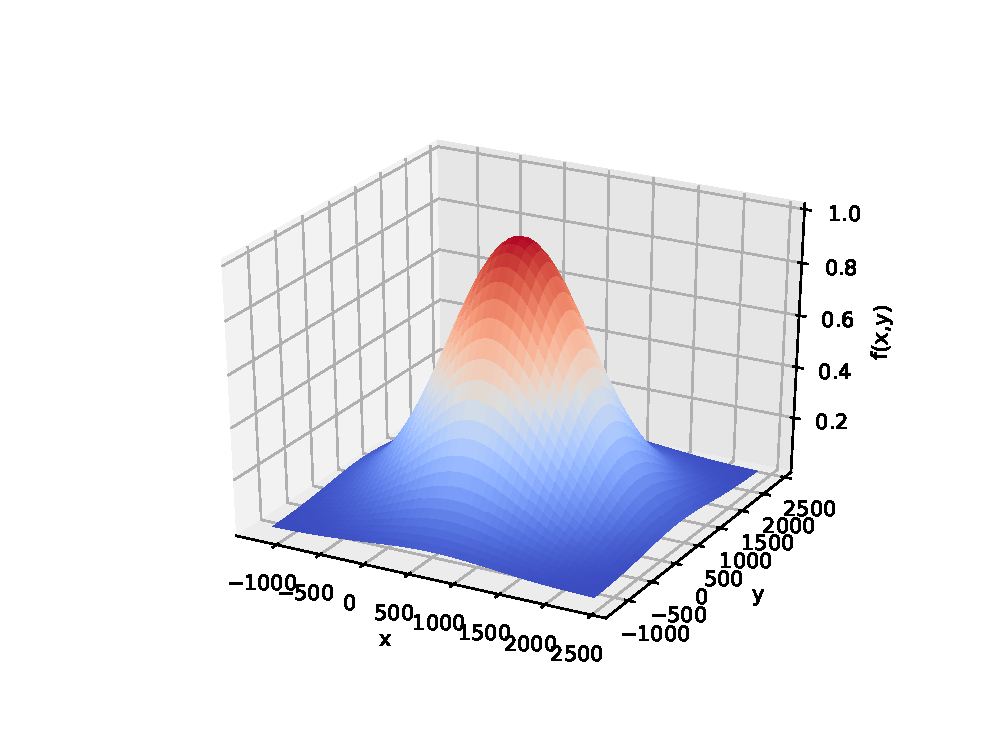
\includegraphics[width=0.45\textwidth]{figures/Gaussiana.eps}
        \label{Fgauss}}
    \subfigure[Curvas de nivel]{
        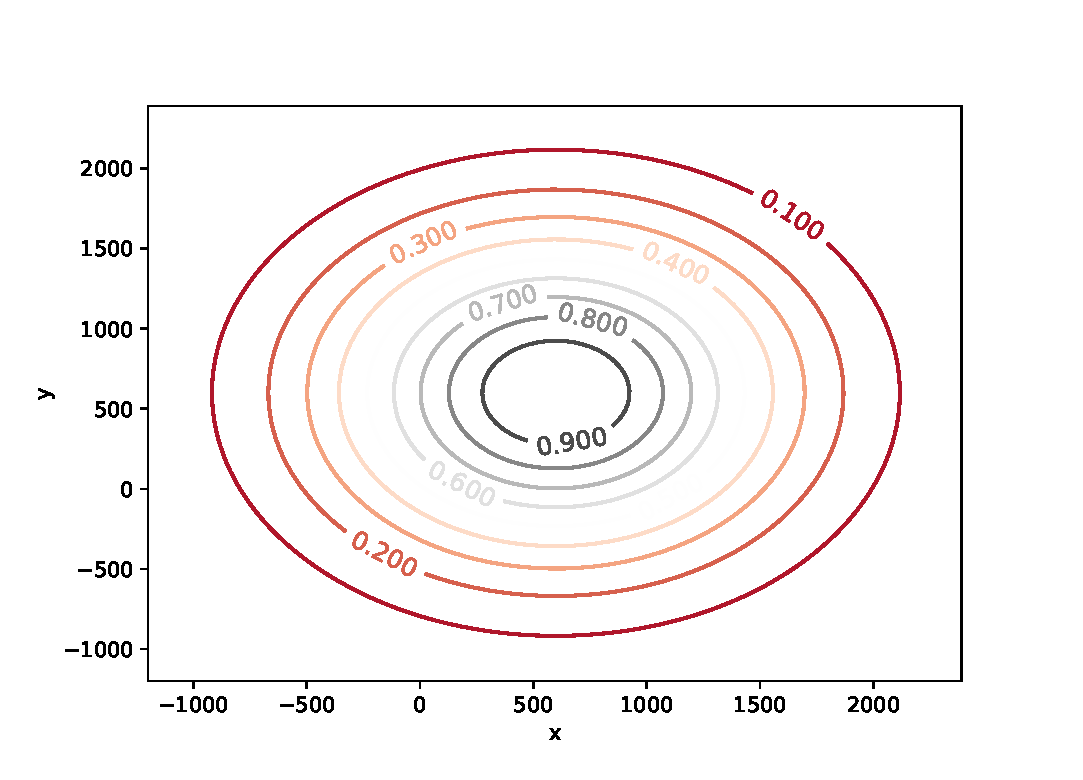
\includegraphics[width=0.45\textwidth]{figures/CurvasNivelGauss.eps}
        \label{CurvasGauss}}
    \caption{Representación de una función lipzchiana}
    \label{FunGauss}
  \end{center}
\end{figure}

Se destaca que toda función lipzchiana a su vez debe ser cuadrática. No obstante, toda función cuadrático no es lipzchiana, un ejemplo de ello es $x^2 = 0$ la cual no esta acotada en un intervalo de la recta. Por ello, se propone la utilización de distribuciones gaussianas para evaluar la eficacia del algoritmo.

Por ende, se define una distribución gaussiana de la siguiente forma:

\begin{equation*}
	f\left(x,y\right)=k·e^{-H}\hspace{10mm}con\hspace{2mm}H=P·S·P^{T}
\end{equation*}

Donde $P=\left[x,y\right]$ son sus coordenadas definidas $\forall_{x,y}\in\mathbb{R}$ y $S=\left[S_x,S_y\right]$ es su desviación siendo una matriz cuadrada y diagonal que mientras más grande sean sus valores más plana será y consecuentemente sus curvas de nivel cubrirán un espacio más amplio, además, su centro va a estar definido como $c=\left[c_x,c_y\right]$.

Finalmente, para la simulación del algoritmo se propuso situar el centro en $c=\left[600,600\right]$, tener una desviación $S=\left[\frac{1000}{sqrt{2}},\frac{1000}{sqrt{2}}\right]$ y finalmente un valor de $k=1$ tal como puede apreciarse en la figura \ref{FunGauss}.

\section{Algoritmo de control de formación circular}

\subsection{Control de formación}

El control de la formación tiene como objetivo evaluar la cooperación y la coordinación en sistemas con múltiples agente, donde su uso recae en impulsarlos a lograr unas restricciones prescritas en sus estados conllevando a formar y mantener una forma geométrica deseada.

Las características esenciales de este tipo de control están relacionadas con la capacidad de detección y la topología de interacción de la red formada por los agentes. Esto conlleva a diferenciar dos tipos de variables:

\begin{itemize}
	\item \textbf{Detectadas:} Especifican la capacidad de detección de los agentes individuales, un ejemplo de ello sería la velocidad u orientación que posee cada agente.
	\item \textbf{Controladas:} Son aquellas relacionadas con la topología de interacción, es decir, sirve para detallar la mejor formación deseada posible que puedan lograr los agentes.
\end{itemize}

\subsection{Descripción general del algoritmo}

El problema de control considera vehículos tipo monociclo con velocidad constante, es decir, solo se actúa sobre la dirección del vehículo a través de giros coordinados actuando sobre el ángulo de inclinación lateral de la aeronave. A esto se le añade la velocidad del viento que altera la velocidad constante propia llevaba por cada agente cuyo marco de coordenadas se encuentra fijado en el centro de una formación circular. Sin embargo, se asumirá que la velocidad del viento es mucho menor que la velocidad deseada, por lo que la velocidad respecto al suelo puede considerarse casi constante durante la misión del vehículo. [2].

El objetivo es describir u  \textbf{algoritmo distribuido para controlar formaciones circulares} de UAV de ala fija con velocidades constantes que actúa sobre el radio del circulo a ser rastreado no sobre la dirección de cada uno de los agentes, es decir, altera la velocidad angular que poseen en torno a un punto central (centro de la circunferencia).\\

\begin{figure}[htb]
\centering
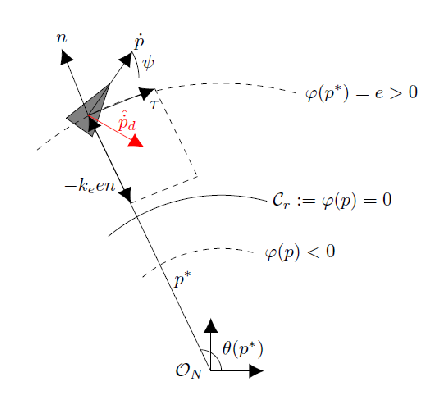
\includegraphics[width=0.6\textwidth]{figures/TA.eps}
\caption{Trayectoria descrita por cada uno de los agentes [Referencia bibliográfica]} \label{fig:Trayectory}
\end{figure}

En resumidas cuentas, cada uno de los robots se encontrarán en un punto $p^*$ cualquiera y ha de converger a un centro definido $C_r$, donde $p^* \cap {C}_r \in \mathbb{R}^{2}$. Consecuentemente, mediante la siguiente ecuación se puede describir los comportamientos adoptados por los agentes.

\begin{equation}\label{Control}
	\varphi\left(p\right)=c_i \Longrightarrow x^2+y^2 - r^2 = c_i
\end{equation}

En donde, $c_i \in \mathbb{R}$ siendo la señal de control que se diseñará y el superindice $i$ denota cada uno de los vehículos/agentes/robots (ver que poner). Se definen dos casos particulares:

\begin{itemize}
	\item Si $c_i$ se hace muy pequeño, el radio tenderá a aumentar y con ello se reduce la velocidad angular.
	\item Si $c_i$ se hace muy grande, el radio tenderá a disminuir y con ello se aumenta la velocidad angular.
\end{itemize}

Ambos casos tienen como objetivo converger a la formación circular definida previamente. Finalmente, en esta sección únicamente se trato al algoritmo de manera simplificada dado que más adelante, en el capitulo 4, se dará una descripción más detallada de este, en donde se verán dos formas de consenso entre los agentes, el comportamiento propio descrito para cada uno de ellos o el criterio de convergencia de los agentes.

\section{Acción conjunta de ambos algoritmos}

\subsection{Algoritmo de ascenso de gradiente}

Hasta el momento únicamente se ha comentado sobre la cooperación de los agentes para la disposición de una figura geométrica y simétrica requerida o un algoritmo para la localización de fuentes en el espacio. No obstante, se ha dejado de lado el avance de los agentes, es decir, ha de existir un algoritmo que desplace a todo el enjambre hacia la ubicación de la fuente haciendo uso del gradiente estimado.

Para ello, se utiliza el algoritmo de ascenso de gradiente para desplazar el centro de la formación circular, el cual se encuentra definido de la siguiente forma:

\begin{equation}\label{GA}
	c_{k+1}=c_k+\epsilon\nabla{f}\left(c_k\right)\hspace{10mm}[Referencia bibliografica]
\end{equation}

En donde, $c_k=[x,y]\hspace{2mm}\forall_{x,y}\in\mathbb{R}$ siendo este el centro de la formación circular. Al tratarse de un problema definido como un punto máximo de una función, el avance ha de ser estrictamente positivo, es decir, los valores han de ser cada vez mayores para desplazarte hacia dicho punto. Esto es debido al valor que toma la función siendo $\rightarrow{f}\left(c_k\right)-f\left(c_{k*}\right)<0\rightarrow{f}\left(c_{k*}\right)$ con $\mathrm{\nabla}{f}{\left(c_{k*}\right)}=0$ tal como se vio al inicio del capitulo.

\subsection{Dinámica del sistema}


\begin{figure}[htb]
\centering
\includegraphics[width=0.6\textwidth]{figures/Flujo2.eps}
\caption{Diagrama de flujo que describe la dinámica del sistema [Referencia bibliográfica]} \label{fig:Flujo}
\end{figure}

En la figura \ref{fig:Flujo} se pueden apreciar diferentes colores para diferenciar cada uno de los pasos a seguir antes de llegar a la fuente final, desglosándolos estos serían:

\begin{enumerate}
	\item Se disponen los N agentes en el plano.
	\item Se ejecuta el algoritmo de control de formación circular que cuando los agentes estén dispuestos de manera simétrica, es decir, sus posiciones absolutas no alteren mucho el resultado de la estima del gradiente pasará a la siguiente fase, en caso contrario se quedará esperando que se coloquen en sus sitios.
	\item Al ya estar repartidos alrededor de la formación circular, se hace la estimación del gradiente para obtener la localización de la fuente. En este punto, se dan dos casos que en la figura \ref{fig:Flujo} están referidos como A:
	\begin{itemize}
		\item Si $\widehat{\mathrm{\nabla }}{f}\left(c_{k}\right)\approxeq0$ se está cerca de la fuente conformando una \textbf{solución satisfactoria}.
		\item Si $\widehat{\mathrm{\nabla }}{f}\left(c_{k}\right)>0$ aun están desplazándose para llegar al objetivo.
	\end{itemize}
	\item Si se da la segunda de las situaciones antes planteadas, se ha de desplazar el centro de la formación circular mediante el algoritmo de ascenso de gradiente, tal como se vio en el apartado [hacer referencia al capitulo anterior].
	\item Antes de volver a estimar el gradiente se debe comprobar el paso 2, en caso de permanecer en sus posiciones de la formación directamente partes del paso 3.
\end{enumerate}




\newpage
\thispagestyle{empty}
\mbox{}

\chapter{Estimación del gradiente}
\label{ch:chapter3}

Acá la idea es describir el algoritmo con su desarrollo matemático para que no salga nada de la nada (mas o menos 10-12 paginas en este capitulo).

Se pretende describir un procedimiento para estimar el gradiente de una función "$\widehat{\mathrm{\nabla }}{f}\left(c\right)$", basándose en mediciones locales de múltiples robots situados de manera simétrica en un espacio de 2D. En dicho procedimiento, se consideran N robots distribuidos uniformemente a lo largo de una formación circular con un radio D y un punto central c definido en dos dimensiones.

Partiendo de la ecuación (Ecuación de la expasion de Taylor del inicio, poner el numero), pero haciendo la expansión únicamente hasta el termino de primer orden sobre cada una de las medidas $r_i$ pertenecientes a la función "${f}\left({r}_{i}\right)$".

\begin{equation*}
	f\left(r_{i}\right)-f\left(c\right)=\mathrm{\nabla}{f}\left(c\right)^{T}\left(r_{i}-c\right)+\varphi_{i}\left(D,c\right)
\end{equation*}

Me quede aca, desde aca para abajo es sucio.

En donde $r_{i}=$ es la posición del robot i, ${\boldsymbol{\phi }}_{\boldsymbol{i}}\boldsymbol{=}\frac{\boldsymbol{2}\cdot\boldsymbol{\pi }\cdot\boldsymbol{i}}{\boldsymbol{N}}\boldsymbol{\ }$es el ángulo de rotación, $R_{\phi }$ \underbar{es la matriz de rotación} definida como \textbf{ }$\left[ \begin{array}{cc} {\boldsymbol{c}}_{\boldsymbol{\phi }} & \boldsymbol{-}{\boldsymbol{s}}_{\boldsymbol{\phi }} \\  {\boldsymbol{s}}_{\boldsymbol{\phi }} & {\boldsymbol{c}}_{\boldsymbol{\phi }} \end{array} \right]$\textbf{, }finalmente $e\ =\ {\left[1,0\right]}^T$, por simplicidad no se considera la dinámica de los robots.



\noindent La señal está definida según una función cuadrática $\boldsymbol{\sigma }\boldsymbol{(}\boldsymbol{r}\boldsymbol{)=}{\boldsymbol{r}}^{\boldsymbol{T}}\boldsymbol{\cdot}\boldsymbol{S}\boldsymbol{\cdot}\boldsymbol{r}\boldsymbol{+}{\boldsymbol{p}}^{\boldsymbol{T}}\boldsymbol{\cdot}\boldsymbol{r}\boldsymbol{+}\boldsymbol{q}$ si se tiene una formación de más de 4 robots se asume que la estimación es el gradiente de la función.

\noindent 
\[{\phi }_i={\phi }_{o}+\frac{2\cdot\pi \cdot{i}}{N} \] 

Con ${\phi }_{o}\left(t\right)=w_{o}\cdot{t}$la formación propuesta es adecuada para robots que se mueven en formación circular como vehículos aéreos no tripulados de área.

Problema en cuestión:

Se puede poner de tres formas:

Primera forma:

\begin{equation*}
	\hat{\nabla}{f}\left(c\right):=\frac{2}{{D}^2\cdot{N}}\cdot\sum_{i=1}^{N}f(r_{i})\cdot(r_{i}-c)
\end{equation*}

Donde:

\begin{equation*}
	\hat{\nabla}{f}\left(c\right) = \nabla{f}\left(c\right) + \varphi\left(D,c\right)
\end{equation*}

Segunda forma:

\begin{equation*}
	\frac{2}{{D}^2\cdot{N}}\cdot\sum_{i=1}^{N}f(r_{i})\cdot(r_{i}-c)=\nabla{f}\left(c\right) + \varphi\left(D,c\right)
\end{equation*}


Tercera forma:

\begin{equation*}
	\frac{2}{{D}^2\cdot{N}}\cdot\sum_{i=1}^{N}f(r_{i})\cdot(r_{i}-c)=\underbrace{\nabla{f}\left(c\right) + \varphi\left(D,c\right)}_{:=\hat{\nabla}{f}\left(c\right)}
\end{equation*}


Se tiene una función $f\left(r\right)$, donde $r$ definida en 2 dimensiones, que el gradiente en el punto máximo es 0 ($\mathrm{\nabla }f\left(r^*\right)=0$), pero en el punto del campo escalar será distinto de 0 ($\left(\mathrm{\nabla }\sigma \left(r\right)\neq 0\right),$ obviamente se ha de dar con ``situaciones espaciales'' diferentes lugares ($\forall r\neq r^*$) y finalmente el hessiano estará definido negativamente dado que es un máximo local, es decir, $H_{\sigma (r^*)}<-a\cdot{I}_{p}$ (con a $\mathrm{>}$ 0 e $I_p$ es una matriz identidad perteneciente al espacio $R^{pxp}$.



Parrafos que me pueden servir en algun momento:


Se tienen dos casos ${\left[A\right]}_{\alpha }=A$ si $A\le -\alpha \cdot{I}_{p}$  sino seria  ${\left[A\right]}_{\alpha }=-I_p$, el primero de los casos se utilizará si el centro de formación c está muy alejado de la fuente así se evita que la matriz se defina como semipositiva y tienda a alejar a los robots del punto de interés, además, cuando dicho punto ``c'' está cerca de la fuente se asume entonces que $A<-\alpha \cdot{I}_{p}$

\newpage
\thispagestyle{empty}
\mbox{}

\chapter{Conclusiones y futuras investigaciones}
\label{ch:chapter4}

Al evaluar el comportamiento del sistema completo variando sus parámetros más relevantes y en dos situaciones completamente diferentes se pueden extraer las siguientes conclusiones:

En primer lugar, la operación conjunta de los tres algoritmos satisfacen los objetivos dispuestos en \ref{Objetives} que consistía en determinar la zona de máxima concentración de sustancias en superficies marítimas. Sin embargo, dados los distintos resultados obtenidos se puede deducir que determinar el número de agentes, el radio y hasta el peso correspondiente al avance, se deben elegir con especial cuidado dado que una mala elección de cualquiera de estos tres puede conllevar a que el sistema se ralentice, no sea fiable o incluso que ni llegue al punto de inflexión.

Por otro lado, recopilando todos los resultados gráficos obtenidos se aprecia que el sistema en sí es mucho más sensible al radio de la formación que al número de agentes. Este ultimo llegando a ser incluso despreciable a partir de un valor $N_{max}$, si retomas la referencia \cite{Adicional_Estimacion_1} acota al error de la siguiente forma:

\begin{equation}\label{Depe}
	||\hat{\nabla}f\left(c\right)-\nabla{f}\left(c\right)||\leqslant{D·L}
\end{equation}

En donde, $L$ es un escalar delimitado por $\varphi_i\left(D,c\right)\leq{L\cdot{||r-c||^2}}$. Si bien es cierto que el error depende del radio de la formación D de tal forma que un aumento conlleva a tener más error al darle mayor margen sobre la desigualdad \ref{Depe}. No obstante, el algoritmo a su vez debería de estar acotado por el número de agentes que a pesar de influir en menor medida también deben de tomarse en cuenta para dicha cota.

Un aspecto de vital importancia es el propio avance del algoritmo definido por el ascenso de gradiente. En este se recogen los dos errores dados por la estima de gradiente del algoritmo de búsqueda de fuentes y el error asociado al ángulo entre vecinos adyacentes del algoritmo de control de formación, a su vez se le añade que contiene el valor del peso $\epsilon$. Por lo que si juntas una mala definición de parámetros con los errores acumulados se pueden describir espirales incluso más pronunciadas que las referidas en \ref{Epsilon_Var}.

Tanto en como en \cite{Estimacion_Gradiente} como en \cite{Adicional_Estimacion_1} dan una forma de corregir el error dado por la mala elección del peso $\epsilon$ y las limitaciones apreciadas del algoritmos de ascenso de gradiente. Esto es hacer uso del Newton-Raphson, en el que aprovechas el hessiano de la función para desplazarte sobre su derivada. No obstante, se debe de estimar tal como se hizo con el gradiente pero para ello se ha de definir un vehículo adicional en el centro de la formación dificultado un poco la coordinación entre ellos.

Finalmente, un reto que actualmente se plantea es como dotar a un único vehículo la capacidad de dirigir al enjambre entero sin que el resto sepan absolutamente nada, es decir, solo un único agente posee información sobre el sistema. Esto traducido, por ejemplo, al algoritmo de búsqueda de fuentes sería si solo uno de los vehículos sabe donde esta el gradiente que técnicas habrían que implementar para que el resto de los agentes que conforman al sistema sepan hacia donde tienen que ir sin poseer ningún tipo de información.
%\newpage
\thispagestyle{empty}
\mbox{}

\chapter{Conclusiones}
\label{ch:chapter5}


Acá irían las gráficas de las simulaciones que estoy haciendo actualmente (llevaría de momento 1 de indice + 3-4 introducción + 18-20 (en dos capítulos), 6-8 el capitulo 4 y 6-8 el capitulo de conclusiones, mas la bibliográfica, darían en torno a 40-48).
%\newpage
\thispagestyle{empty}
\mbox{}

\chapter{Parrafor en sucio}
\label{ch:chapter6}


En donde, $\sigma$ es la desviación típica aportando información sobre la variación de la concentración de las sustancias y $\mu$ la media que representa el punto de máxima radiación de la fuente. Un aspecto relevante es que si el centro de la formación se encuentra lo suficientemente cerca de la fuente el argumento de la exponencial tenderá a 0 conllevando a que en torno a dicho punto se tenga la máxima concentración de sustancias.

\begin{figure}[htb]
\centering
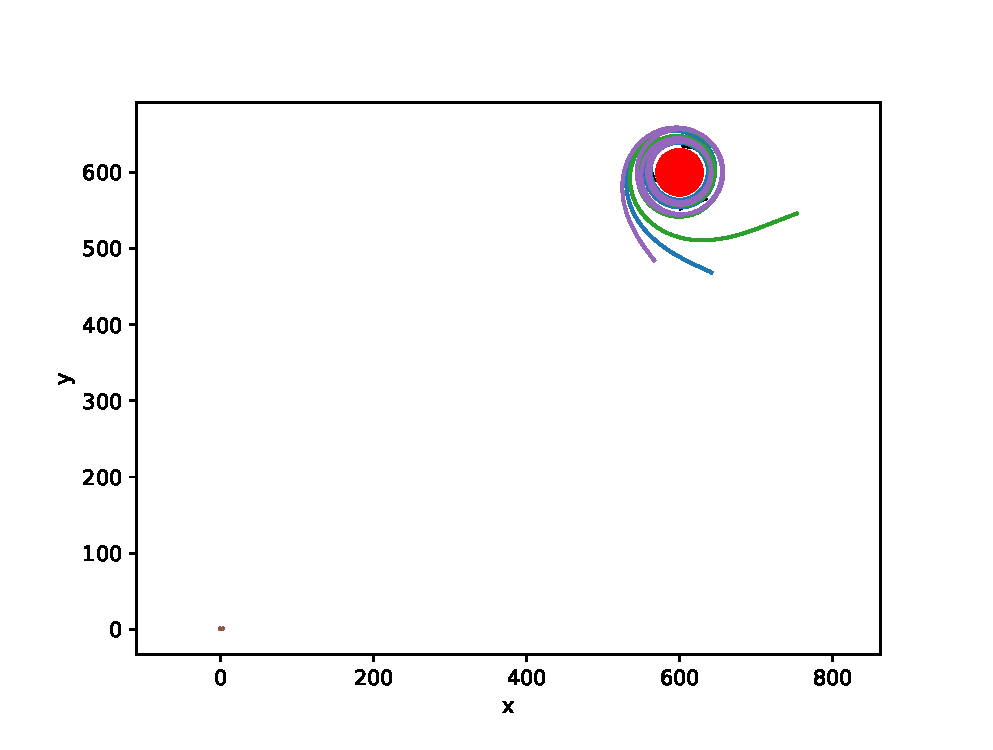
\includegraphics[width=0.85\textwidth]{figures/Coordinacion/Objetivo_Final.eps}
\caption{Vehículos dispuestos en torno a la formación. El punto rojo representa el circulo al que quieren converger y las diferentes líneas que giran en torno a dicho punto son cada una de las trayectorias de los vehículos.} \label{Ejemplo_Coordinacion}
\end{figure}

\begin{figure}[htb]
\centering
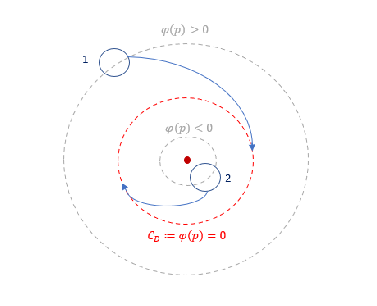
\includegraphics[width=0.60\textwidth]{figures/Pruea_Coordinacion.eps}
\caption{Ejemplo del algoritmo de control de formación} \label{Ejemplo_Coordinacion}
\end{figure}

No obstante, el algoritmo a su vez debería de estar acotado por el número de agentes que a pesar de influir en menor medida también deben de tomarse en cuenta para dicha cota.


% +-------------------------------------------------------------------------+
% | References                                                              |
% +-------------------------------------------------------------------------+

% +-------------------------------------------------------------------------+
% | In order for WinEDT to index references correctly, it has to know where |
% | the file resides.  The following command is prefaced by %, and will be  |
% | ignored completely by LaTeX.  However, WinEDT will use this line to     |
% | access the external .bib bibliography file.  Also note that WinEDT can  |
% | read file path names with either "\" or "/" - LaTeX, however, doesn't   |
% | like "\", so it's easier to store a path name in the "Unix" style.      |
% +-------------------------------------------------------------------------+

%Included for Gather Purpose only.  Do NOT uncomment:
%input "references.bib"

% +--------------------------------------------------------------------+
% | This template uses the BibTeX program to format references.  The
% | 3 lines below create a separate Bibliography section and add
% | an entry for "Bibliography" to the Table of Contents.  The actual
% | data for your references (author, title, journal, date, etc.) are
% | entered in the references.bib file.  See that file for information
% | on how to enter references.
% +--------------------------------------------------------------------+
%\newpage
\thispagestyle{empty}
\mbox{}
\begin{thebibliography}{3}

\bibitem{Estimacion_Gradiente}
L. Briñón-Arranz, L. Schenato, Member, IEEE, and A. Seuret. Distributed Source Seeking via a Circular Formation of Agents Under Communication Constrains. IEEE Trans. on Control of Network Systems, vol. 3, no. 2, June 2014.

\bibitem{Control_Formacion}
H. Garcia de Marina, Z. Sun, M. Bronz, and G. Hettenberger. Ciruclar formation control of fixed-wing UAVs with constant speeds. Conference Paper - September 2017.

\bibitem{Adicional_Estimacion_1}
L. Briñón-Arranz, A. Renzaglia, and L. Schenato. Multi-Robot Symmetric Formations for Gradient and Hessian Estimation with Application to Source Seeking. IEEE Trans. on Robotics, IEEE, 2019, 35 (3), pp.782-789.

\bibitem{Otra_Coorporativa}
L. Briñon Arranz, A. Seuret, and C. Canudas de Wit. Cooperative Control Design for Time-Varying Formations of Multi-Agent Systems. IEEE Transactions on Automatic Control,Institute of Electrical and Electronics Engineers (IEEE), 2014, 59 (8), pp.2283-2288.



\end{thebibliography}

%\bibdata{references}
%\bibliographystyle{abbrv}
\phantomsection
\bibliographystyle{ieeetr}
%\bibliographystyle{unsrt}
\bibliography{references}
\addcontentsline{toc}{chapter}{Bibliografía}


% +--------------------------------------------------------------------+
% | Finally, we generate the appendix.  To add or delete appendices,
% | add or remove the line
% |
% |     \input{appendixX.tex}
% |
% | where "X" is the letter designation of the Appendix (A, B, C, etc.)
% | You should have one \input{appendixX.tex} line and a corresponding
% | file appendixX.tex for each appendix.                                 |
% +--------------------------------------------------------------------+

%\appendix
%\newpage
\thispagestyle{empty}
\mbox{}

\chapter{Introduction}
\label{appendixA}


%\newpage
\thispagestyle{empty}
\mbox{}

\chapter{Conclusions}
\label{apenddixB}


%\newpage
\thispagestyle{empty}
\mbox{}

\chapter{Instrucciones de instalación}
\label{apenddixC}





%\newpage
\thispagestyle{empty}
\mbox{}

\chapter{JSON. Mensaje de ejemplo}
\label{appendixD}


%\clearpage
\thispagestyle{empty}
\mbox{}

\chapter{Código LUA. Comunicación $I^2C$}
\label{apenddixE}


%\clearpage
\thispagestyle{empty}
\mbox{}

\chapter{Código LUA. Script principal}
\label{apenddixF}



\end{document}
